\subsection*{Scheduling}
\underline{Timing constraints:}\\
Deadline: D\\
Arrival time: A\\
Release time: R\\
Finish time: F\\
Computation time: C\\
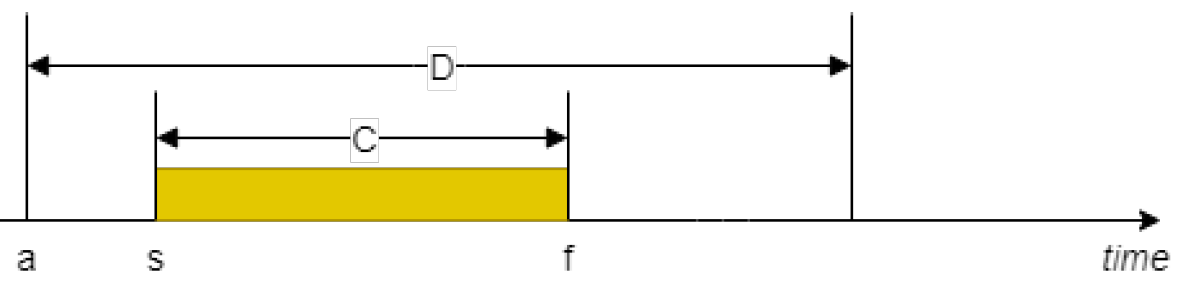
\includegraphics[width=\columnwidth]{images/timing_constraints.png}
\textit{Task response time} $=f-a$ ou $f-r$\\
\textit{Maximum lateness} $=\max_i(f_i-d_i)$\\
\textit{Maximum number of late tasks}
$=\sum_{i=1}^{n} \text{miss}(f_i)=
    \begin{cases}
        0 & \text{if } f_i \leq d_i \\
        1 & \text{otherwise}
    \end{cases}$\\
\textit{Schedulability:} $U=\sum_{i=1}^{n} \frac{C_i}{T_i} \leq 1$\\
Can be increased by increasing task computation times or by decreasing their periods.\\
\textbf{Time cyclic scheduling:}\\
Divide the temporal axis into slots of equal length (length = Minor Cycle).
The optimal length of the Minor Cycle is the GCD (=plus grand diviseur commun) of the periods.
The optimal length of the Major Cycle is the LCM (=plus petit multiple commun) of the periods.
If tasks cannot be split into sub-tasks, then a set of tasks is schedulable if
the sum of execution times within each time slot is less or equal to the Minor
Cycle.\\
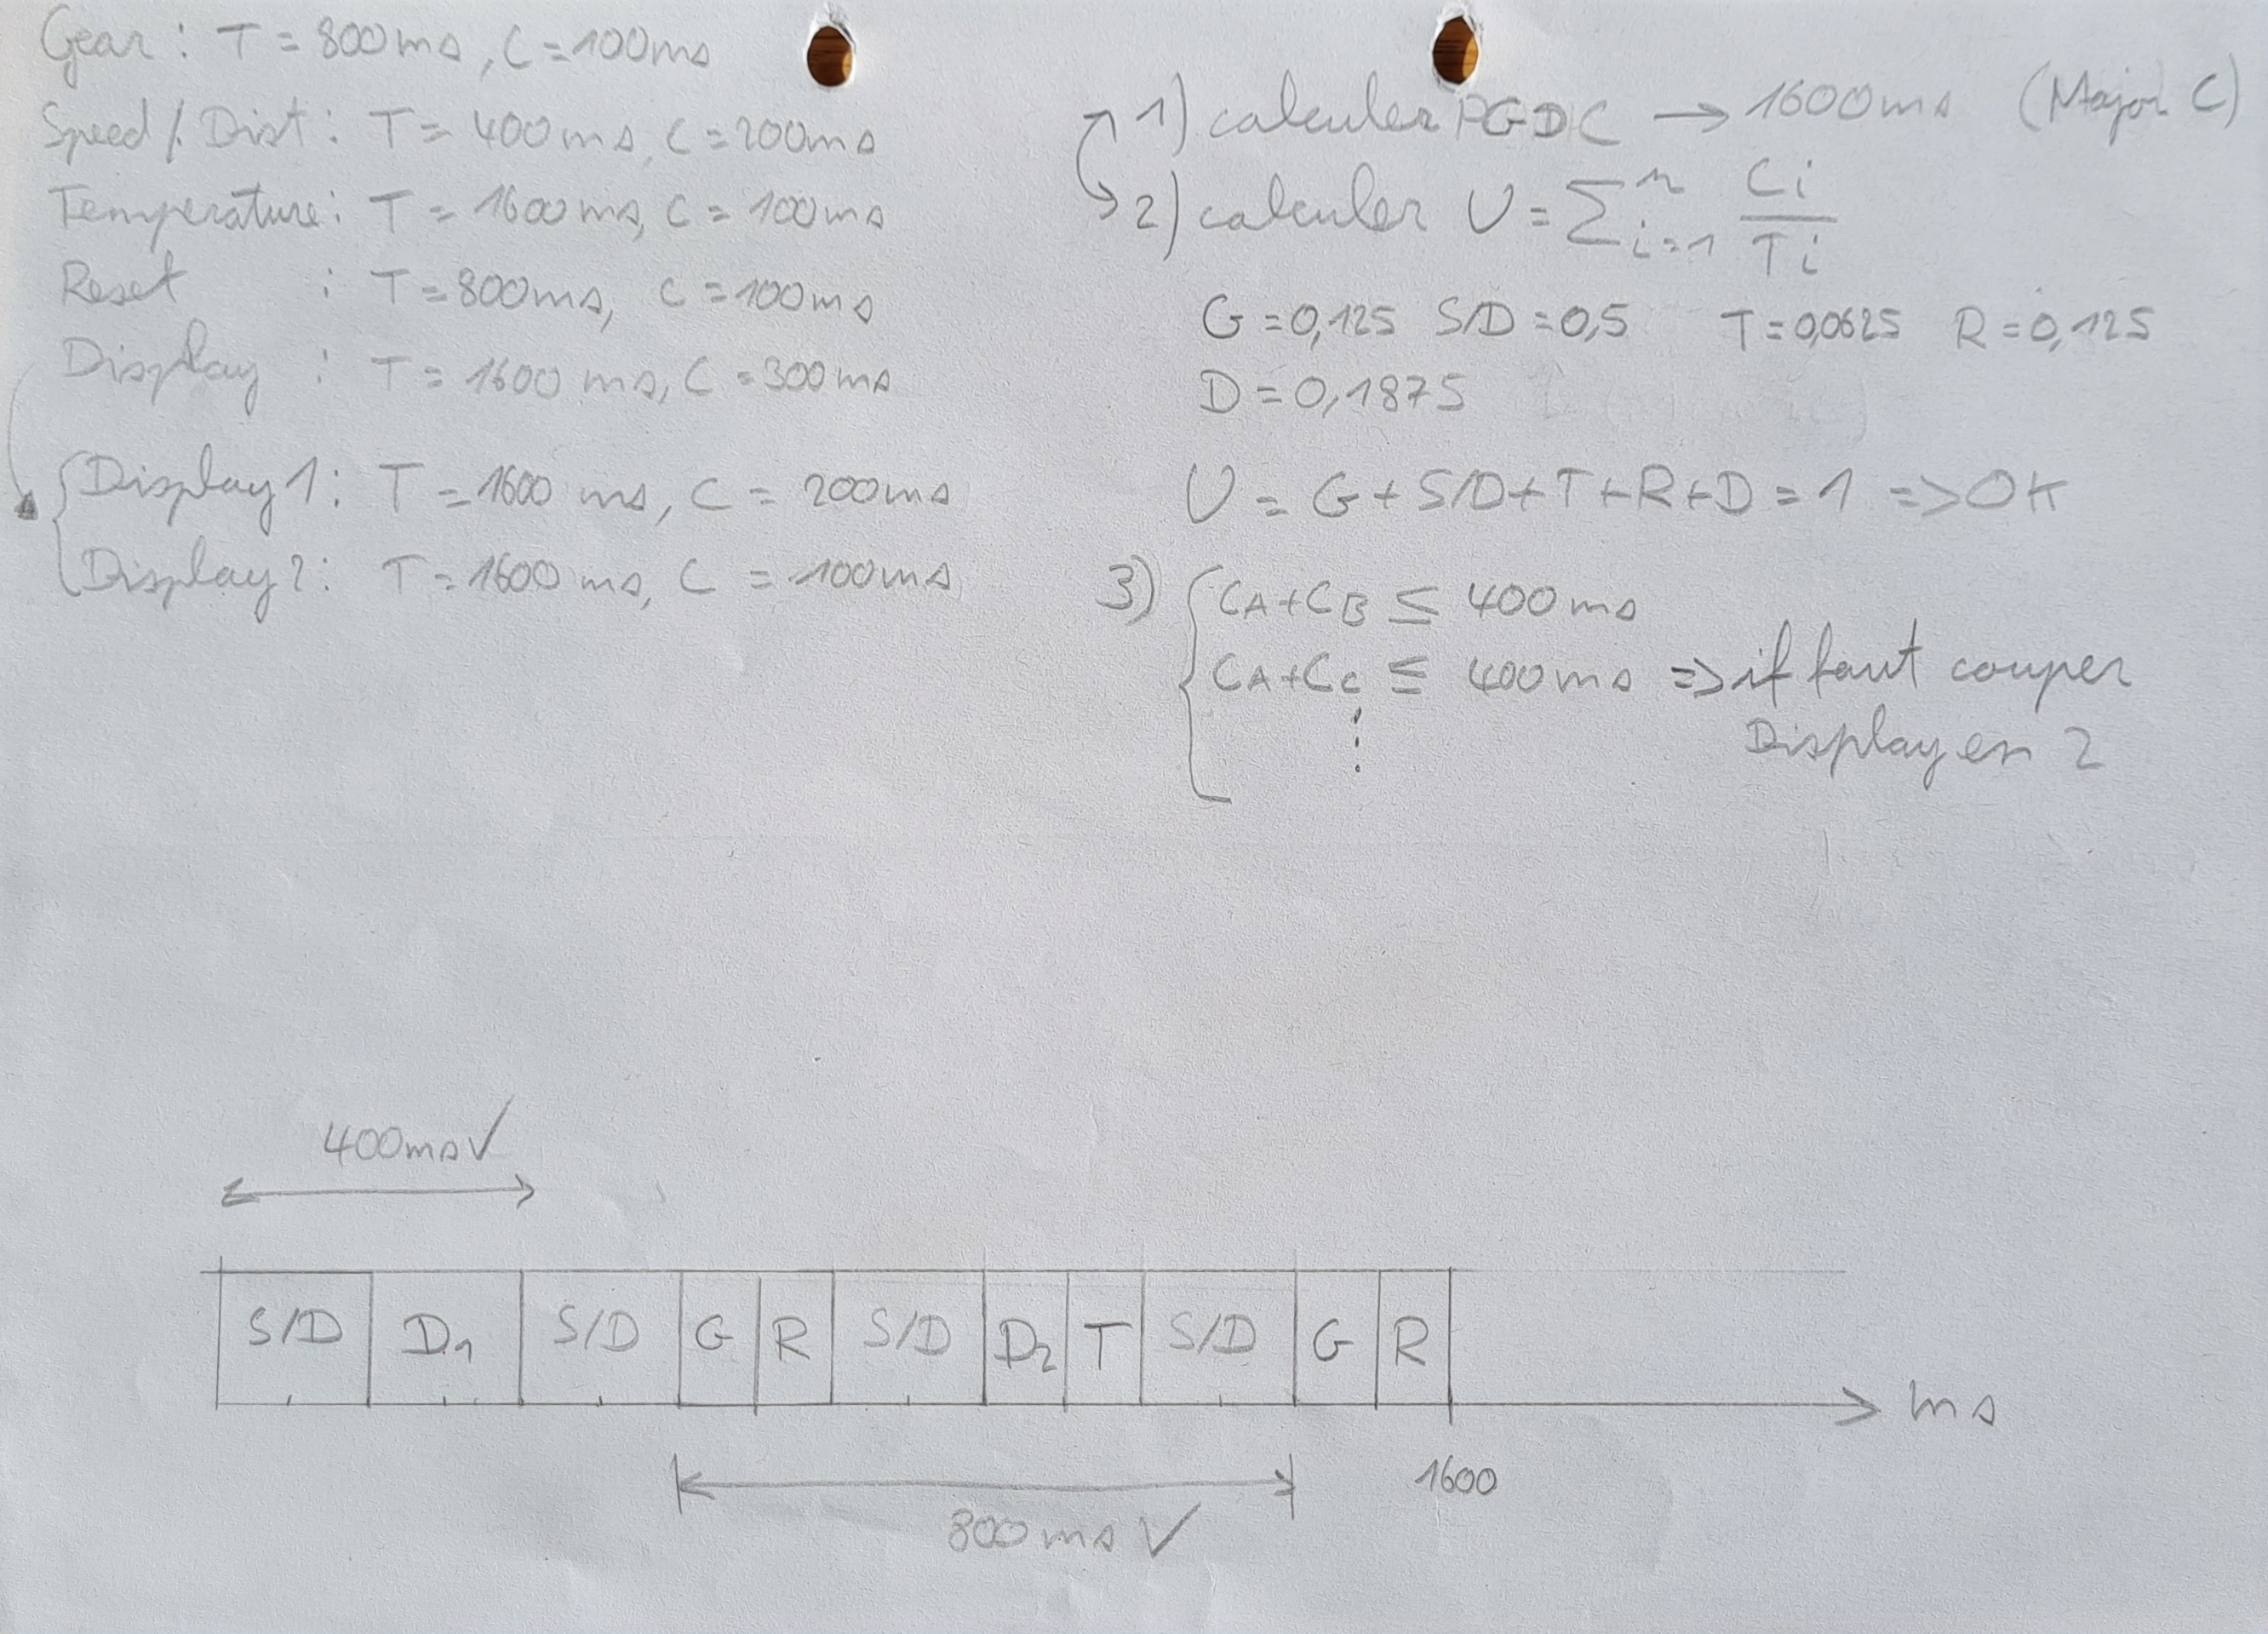
\includegraphics[width=\columnwidth]{images/time_cyclic_scheduling.jpg}
Advantages:
\begin{itemize}
    \item Easy to implement
    \item Predictable
    \item No need for a scheduler
\end{itemize}
Disadvantages:
\begin{itemize}
    \item Always run the same schedule
    \item The polling rate is limited by 1/maximum delay.
    \item The program must continually check the status of every device
    \item This approach scales badly
\end{itemize}
\textbf{Event-driven systems:}\\
Handling events is done using interrupts. Interrupts can be prioritized.
Interrupts can be masked: switched off if not needed or likely to get in the way of more
important activity. Interrupts can be nested. The location of the ISR in memory can be selected.\\
%put two images side by side 
\begin{minipage}{.49\columnwidth}
    \centering
    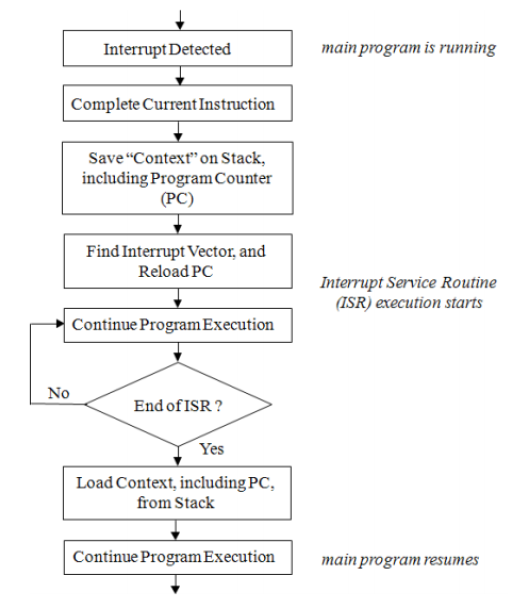
\includegraphics[width=\linewidth]{images/interrupt1.png}
\end{minipage}
\begin{minipage}{.49\columnwidth}
    \centering
    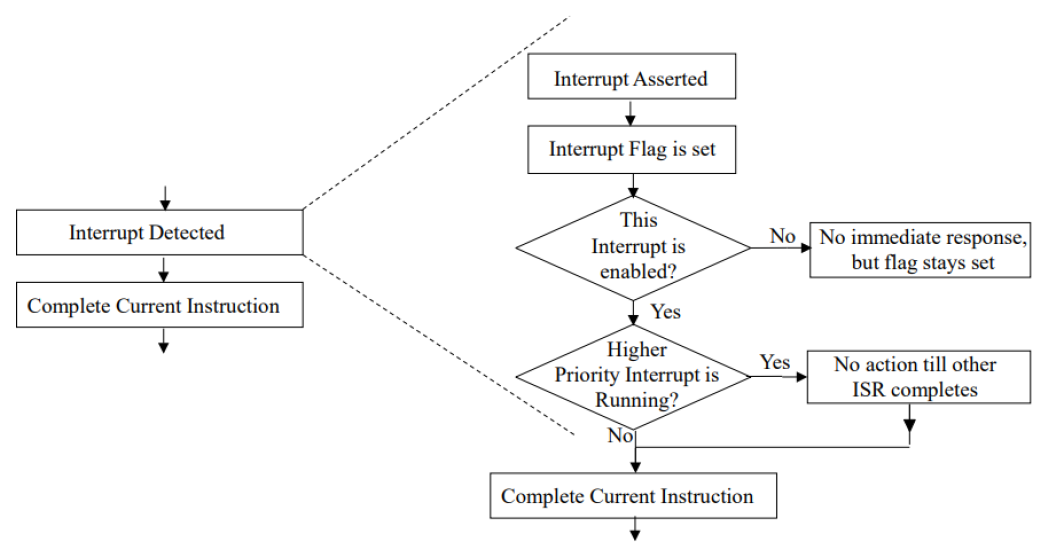
\includegraphics[width=\linewidth,height=\linewidth,keepaspectratio=false]{images/interrupt2.png} % set height to \linewidth
\end{minipage}\\
\textbf{Dynamic scheduling:}\\
Allows task scheduling to be computed dynamically online based on importance or any other
criteria such as task deadline, duration, or creation time.\\
\underline{Task preemption:}\\
Exception handling/interrupt may need to preempt existing tasks.
Suspend a running task and insert it in the ready queue. Schedule tasks based on their
priority/importance. Improve efficiency.\\
Advantages:
\begin{itemize}
    \item Better response time
    \item Can do more processing
    \item Can lower processor speed, saving money and power
\end{itemize}
Disadvantages:
\begin{itemize}
    \item More complicated programming
    \item More memory.
    \item Introduces vulnerability
\end{itemize}
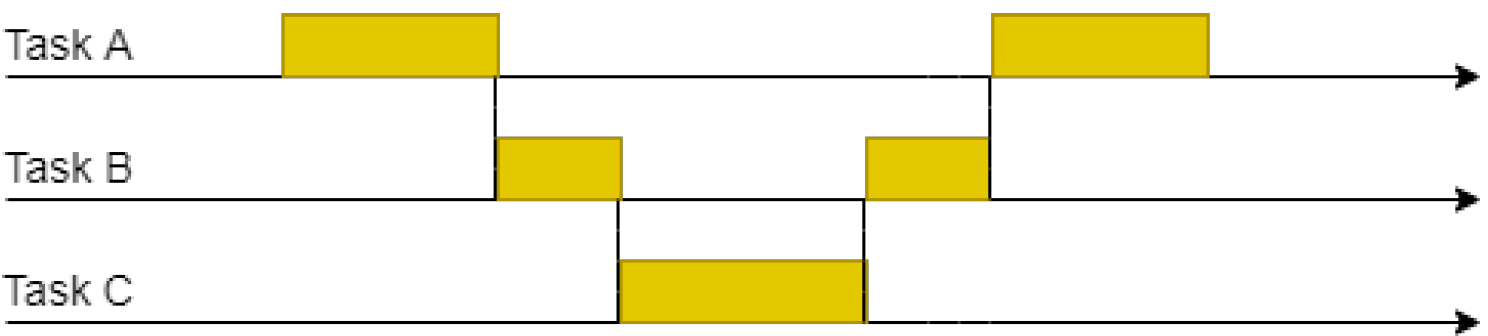
\includegraphics[width=\columnwidth]{images/preemption.png}
\underline{Rate Monotonic Scheduling:}\\
Tasks with higher request rates/shorter periods have higher priorities.
Fixed periods means fixed priorities. Is optimal among fixed-priority algorithms.
\textit{Schedulability:} $U=\sum_{i=1}^{n} \frac{C_i}{T_i} \leq n(2^{\frac{1}{n}}-1)$\\
\underline{Earliest Deadline First:}\\
Tasks with earlier deadlines have higher priorities.
Priorities are dynamic since absolute deadlines of periodic tasks vary over time.
\textit{Schedulability:} $U=\sum_{i=1}^{n} \frac{C_i}{T_i} \leq 1$\\
